%% Verification Report: Ice Ih MC Simulation
%  Content:
%  1. Dimensionless verification (T* = kBT/epsilon)
%  2. Exact enumeration for small N
%  3. Finite-size scaling and extrapolation
%  4. Conclusions on algorithm reliability

\documentclass[12pt, a4paper]{article}

\usepackage[utf8]{inputenc}
\usepackage[T1]{fontenc}
\usepackage[margin=2.5cm]{geometry}
\usepackage{amsmath, amssymb}
\usepackage{graphicx}
\usepackage{booktabs}
\usepackage{array}
\usepackage{float}
\usepackage{hyperref}
\usepackage[dvipsnames]{xcolor}
\usepackage{tcolorbox}
\tcbuselibrary{theorems, breakable, skins}
\usepackage{fancyhdr}
%\usepackage{microtype}
\usepackage{caption}
\usepackage{setspace}
\usepackage{amsthm}

\theoremstyle{plain}
\newtheorem{proposition}{Proposition}[section]

\theoremstyle{definition}
\newtheorem{remark}{Remark}[section]

\hypersetup{
    colorlinks=true, linkcolor=NavyBlue,
    citecolor=ForestGreen, urlcolor=MidnightBlue,
}

\pagestyle{fancy}
\fancyhf{}
\rhead{\small Verification Report -- Ice Ih MC Simulation}
\lhead{\small Yi Tang}
\cfoot{\thepage}
\setlength{\headheight}{14pt}

%-- Highlighted box
\newtcolorbox{keyresult}[1][]{
    enhanced, breakable,
    colback=blue!5!white, colframe=NavyBlue,
    fonttitle=\bfseries, title=Key Result, #1
}
\newtcolorbox{conclusion}[1][]{
    enhanced, breakable,
    colback=green!5!white, colframe=ForestGreen,
    fonttitle=\bfseries, title=Conclusion, #1
}

\newtcolorbox{puzzle}[1][]{
    enhanced, breakable,
    colback=red!5!white, colframe=Red,
    fonttitle=\bfseries, title=Puzzle, #1
}

%-- Math macros
\newcommand{\COH}{C_\mathrm{OH}^B}
\newcommand{\eps}{\varepsilon}
\newcommand{\kB}{k_{\mathrm{B}}}
\newcommand{\Nocc}{N_\mathrm{occ}}
\newcommand{\Tstar}{T^*}
\newcommand{\avgE}[1]{\langle #1 \rangle}

%================================================================
\begin{document}
%================================================================

%-- Title
\begin{titlepage}
\centering
\vspace*{2cm}
{\LARGE\bfseries Verification Report}\\[0.8em]
{\large Ice Ih Basal Surface: MC Simulation of Proton Order}\\[0.5em]
{\normalsize Algorithm Verification via Dimensionless Analysis\\
and Exact Enumeration}
\vspace{1.5cm}

{\large Yi Tang}\\[0.4em]
{\normalsize \today}

\vspace{2cm}
% \begin{abstract}
% \noindent
% This report documents the verification strategy for the
% Kawasaki--Metropolis Monte Carlo simulation of proton ordering
% on the ice Ih basal surface.
% Two independent verification methods are employed.
% First, results are plotted in dimensionless units
% $\Tstar = \kB T/\eps$, which removes any dependence on the
% specific value of $\eps$ and allows a direct comparison between
% MC and exact enumeration on the same axis.
% Second, exact enumeration of the full state space is performed
% for small lattices ($N \leq 24$), providing a parameter-free
% reference against which the MC algorithm is validated.
% Finite-size scaling is then used to study how results depend on
% system size and to extrapolate toward the thermodynamic limit.
% The combination of these two methods verifies that the algorithm
% is correct independently of the choice of $\eps$.
% \end{abstract}
\end{titlepage}

\tableofcontents
\newpage

%================================================================
\section{Motivation and Verification Strategy}
%================================================================

The simulation computes the equilibrium order parameter
$\avgE{\COH}$ as a function of temperature $T$ using a single-trajectory
Kawasaki--Metropolis Markov chain with sequential annealing.
Two potential sources of error must be distinguished:

\begin{enumerate}
    \item \textbf{Algorithm errors}: bugs in the MC step, the
          $\Delta E$ calculation, the $\COH$ measurement, or the
          neighbour list construction.
    \item \textbf{Parameter errors}: an incorrect value of the
          nearest-neighbour repulsion energy $\eps$.
\end{enumerate}

These two sources affect the results differently.
An algorithm error distorts the \emph{shape} of the
$\avgE{\COH}$--$\Tstar$ curve.
A parameter error shifts the curve \emph{horizontally} when
plotted against physical temperature $T$ (K), because the
physical temperature scale is set by $\eps/\kB$.

The verification strategy therefore proceeds in two steps:

\begin{enumerate}
    \item \textbf{Dimensionless comparison}: plot all results
          against $\Tstar = \kB T/\eps$.
          In these units, both MC and exact enumeration must
          produce the same curve if the algorithm is correct,
          regardless of the value of $\eps$.
    \item \textbf{Exact enumeration}: for small lattices
          ($N \leq 24$), compute $\avgE{\COH}(\Tstar)$ by direct
          summation over all states in $\Omega$, with no
          statistical error and no dependence on algorithm choices.
          Agreement between MC and exact enumeration in dimensionless
          units proves the algorithm is correct.
\end{enumerate}

%================================================================
\section{Dimensionless Formulation}
%================================================================

\subsection{Dimensionless temperature}

The Hamiltonian contains a single energy scale $\eps$:
\[
    H(\sigma) = \eps \sum_{\langle ij \rangle} t_i t_j.
\]
Defining the dimensionless temperature
\[
    \Tstar = \frac{\kB T}{\eps},
\]
the Boltzmann weight becomes $e^{-H/(\eps \Tstar)}$, and
$\avgE{\COH}$ is a function of $\Tstar$ alone:
\[
    \avgE{\COH}(\Tstar) =
    \frac{\displaystyle\sum_{\sigma\in\Omega}
          \COH(\sigma)\,e^{-\sum_{\langle ij \rangle} t_i t_j/(\Tstar)}}
         {\displaystyle\sum_{\sigma\in\Omega}
          e^{-\sum_{\langle ij \rangle} t_i t_j/(\Tstar)}}.
\]
This function is uniquely determined by the lattice geometry
and the constraint $\Nocc = N/2$; it does not depend on $\eps$.

% \subsection{Wannier approximation in dimensionless units}

% The Wannier analytic approximation becomes
% \[
%     \avgE{\COH}_{\mathrm{Wannier}}(\Tstar)
%     \approx
%     2 + \frac{6\,e^{-2/\Tstar}}{1 + 3\,e^{-2/\Tstar}}.
% \]
% This expression is independent of $\eps$ and provides a
% reference curve derived from an infinite, unconstrained system.
% Deviations from this curve in the exact enumeration results
% are physical (finite-size effects and the $N/2$ constraint),
% not algorithmic errors.

\subsection{Exact high-temperature limit}

\begin{proposition}[High-Temperature Limit]
\label{prop:highT}
In the limit $T \to \infty$, the equilibrium order parameter
satisfies
\begin{equation}
    \langle \COH \rangle_{T\to\infty}
    = \frac{6(\Nocc - 1)}{N - 1} = 3\left(1-\frac{1}{N-1}\right).
    \label{eq:highT_limit}
\end{equation}
\end{proposition}

\begin{proof}
As $T \to \infty$, the inverse temperature $\beta = 1/\kB T \to 0$,
so the Boltzmann weight $e^{-\beta H(\sigma)} \to 1$ uniformly
over $\Omega$.
The equilibrium distribution therefore converges to the uniform
distribution on $\Omega$:
\[
    \pi(\sigma) \;\to\; \frac{1}{|\Omega|}
    \qquad \forall\,\sigma \in \Omega.
\]

\textbf{Step 1: Rewrite $\COH$ as a sum.}
By definition,
\[
    \COH(\sigma)
    = \frac{1}{\Nocc}
      \sum_{i=1}^{N} \sum_{j \in \partial i} t_i(\sigma)\, t_j(\sigma),
\]
where $t_i(\sigma) \in \{0,1\}$ is the occupation of site $i$
and $\partial i$ denotes its six nearest neighbours.
Taking the expectation under the uniform distribution,
\[
    \langle \COH \rangle_{T\to\infty}
    = \frac{1}{\Nocc}
      \sum_{i=1}^{N} \sum_{j \in \partial i}
      \mathbb{E}[t_i\, t_j].
\]

\textbf{Step 2: Compute $\mathbb{E}[t_i t_j]$.}
Since $t_i t_j = 1$ if and only if both $i$ and $j$ are occupied,
\[
    \mathbb{E}[t_i t_j]
    = P(t_i = 1 \text{ and } t_j = 1).
\]
Under the uniform distribution on $\Omega$, the number of
configurations in which both $i$ and $j$ are occupied is
$\binom{N-2}{\Nocc - 2}$ (place the remaining $\Nocc-2$ protons
on the remaining $N-2$ sites).
Hence
\[
    \mathbb{E}[t_i t_j]
    = \frac{\dbinom{N-2}{\Nocc-2}}{\dbinom{N}{\Nocc}}
    = \frac{(N-2)!\,\Nocc!\,(N-\Nocc)!}{(N_{occ}-2)!\,(N-\Nocc)!\,N!}
    = \frac{\Nocc(\Nocc-1)}{N(N-1)}.
\]

\textbf{Step 3: Evaluate the double sum.}
Each site $i$ has exactly 6 nearest neighbours, so
\[
    \sum_{i=1}^{N} \sum_{j \in \partial i}
    \mathbb{E}[t_i t_j]
    = 6N \cdot \frac{\Nocc(\Nocc-1)}{N(N-1)}
    = \frac{6\Nocc(\Nocc-1)}{N-1}.
\]

\textbf{Step 4: Conclude.}
Dividing by $\Nocc$,
\[
    \langle \COH \rangle_{T\to\infty}
    = \frac{1}{\Nocc} \cdot \frac{6\Nocc(\Nocc-1)}{N-1}
    = \frac{6(\Nocc-1)}{N-1} = 3\left(1-\frac{1}{N-1}\right). \qedhere
\]
\end{proof}

% \begin{remark}
% An equivalent and more intuitive derivation uses conditional
% probability.
% Under the uniform distribution, the probability that site $j$
% is occupied \emph{given} that site $i$ is occupied equals
% \[
%     P(t_j = 1 \mid t_i = 1) = \frac{\Nocc - 1}{N - 1},
% \]
% since, having fixed one proton at $i$, the remaining $\Nocc - 1$
% protons are uniformly distributed over the remaining $N-1$ sites.
% Each occupied site has 6 neighbours, so
% \[
%     \langle \COH \rangle_{T\to\infty}
%     = 6 \cdot P(t_j = 1 \mid t_i = 1)
%     = \frac{6(\Nocc-1)}{N-1}.
% \]
% \end{remark}

\begin{remark}
For the two lattice sizes used in this study:
\begin{align*}
    N = 24,\; \Nocc = 12 &:\quad
    \langle \COH \rangle_{T\to\infty}
    = \frac{6 \times 11}{23} \approx 2.8696, \\[4pt]
    N = 48,\; \Nocc = 24 &:\quad
    \langle \COH \rangle_{T\to\infty}
    = \frac{6 \times 23}{47} \approx 2.9362.
\end{align*}
Both values can be verified directly by setting $\varepsilon = 0$
in the MC simulation (all moves accepted, uniform sampling of
$\Omega$) or by reading off the $T^* \to \infty$ limit of the
exact enumeration curve.
\end{remark}



%================================================================
\section{Exact Enumeration}
%================================================================

\subsection{Feasibility}

The state space $\Omega$ has size $\binom{N}{\Nocc}$.
Table~\ref{tab:omega} lists the sizes for the lattices studied.

\begin{table}[H]
\centering
\caption{State space sizes for candidate lattices.
         Only lattices with $|\Omega| \lesssim 3\times10^6$
         are enumerated exactly.}
\label{tab:omega}
\begin{tabular}{lrrrc}
\toprule
Lattice & $N$ & $\Nocc$ & $|\Omega| = \binom{N}{\Nocc}$ & Enumerated? \\
\midrule
% $3\times4$ & 12 & 6  & 924             & Yes \\
$4\times4$ & 16 & 8  & 12{,}870        & Yes \\
% $5\times4$ & 20 & 10 & 184{,}756       & Yes \\
$6\times4$ & 24 & 12 & 2{,}704{,}156   & Yes \\
$8\times6$ & 48 & 24 & $\approx 4.5\times10^{12}$ & No \\
\bottomrule
\end{tabular}
\end{table}

For $N=48$, direct enumeration requires storing
$\approx 4.5\times10^{12}$ states, which exceeds available
memory and computation time.
However, if the algorithm is verified correct on $N\leq 24$,
the same code applied to $N=48$ is equally reliable,
since the algorithm does not depend on system size.

\subsection{Exact enumeration procedure}

For each lattice:
\begin{enumerate}
    \item Generate all $\binom{N}{\Nocc}$ configurations
          $\sigma \in \Omega$ using \texttt{nchoosek}.
    \item For each $\sigma$, compute:
          \[
              H(\sigma) = \frac{\eps}{2}
              \sum_{i=1}^{N} t_i \sum_{k=1}^{6}
              t_{\partial_k(i)},
          \]
          where $\partial_k(i)$ is the $k$-th neighbour of site
          $i$ from the precomputed neighbour list.
          The factor $1/2$ corrects for double-counting.
    \item Compute $\COH(\sigma)$ from the same neighbour list.
    \item For each $\Tstar$, compute the exact thermal average:
          \[
              \avgE{\COH}(\Tstar)
              = \frac{\sum_s \COH(\sigma_s)\,
                      e^{-H(\sigma_s)/(\eps\Tstar)}}
                     {\sum_s e^{-H(\sigma_s)/(\eps\Tstar)}}.
          \]
\end{enumerate}

\subsection{Verification of limiting cases}

Before computing the full temperature dependence, the following
exact checks are performed for each lattice:

\begin{itemize}
    \item \textbf{Ground state}: the minimum-energy state must
          be the stripe phase with $\COH = 2.0$ exactly.
    \item \textbf{High-temperature limit}: as $\Tstar\to\infty$,
          the exact enumeration must converge to
          equation~\eqref{eq:highT_limit}.
          Table~\ref{tab:checks} reports these values.
\end{itemize}

\begin{table}[H]
\centering
\caption{Verification of limiting cases from exact enumeration.}
\label{tab:checks}
\begin{tabular}{lrrrr}
\toprule
Lattice & $N$ & Ground state $\COH$ & High-$T$ limit (theory)  \\
\midrule
$3\times4$ & 12 & 2.000000 & $6\times5/11 = 2.7273$  \\
$4\times4$ & 16 & 2.000000 & $6\times7/15 = 2.8000$  \\
$5\times4$ & 20 & 2.000000 & $6\times9/19 = 2.8421$ \\
$6\times4$ & 24 & 2.000000 & $6\times11/23 = 2.8696$  \\
\bottomrule
\end{tabular}
\end{table}

\begin{figure}
    \center
    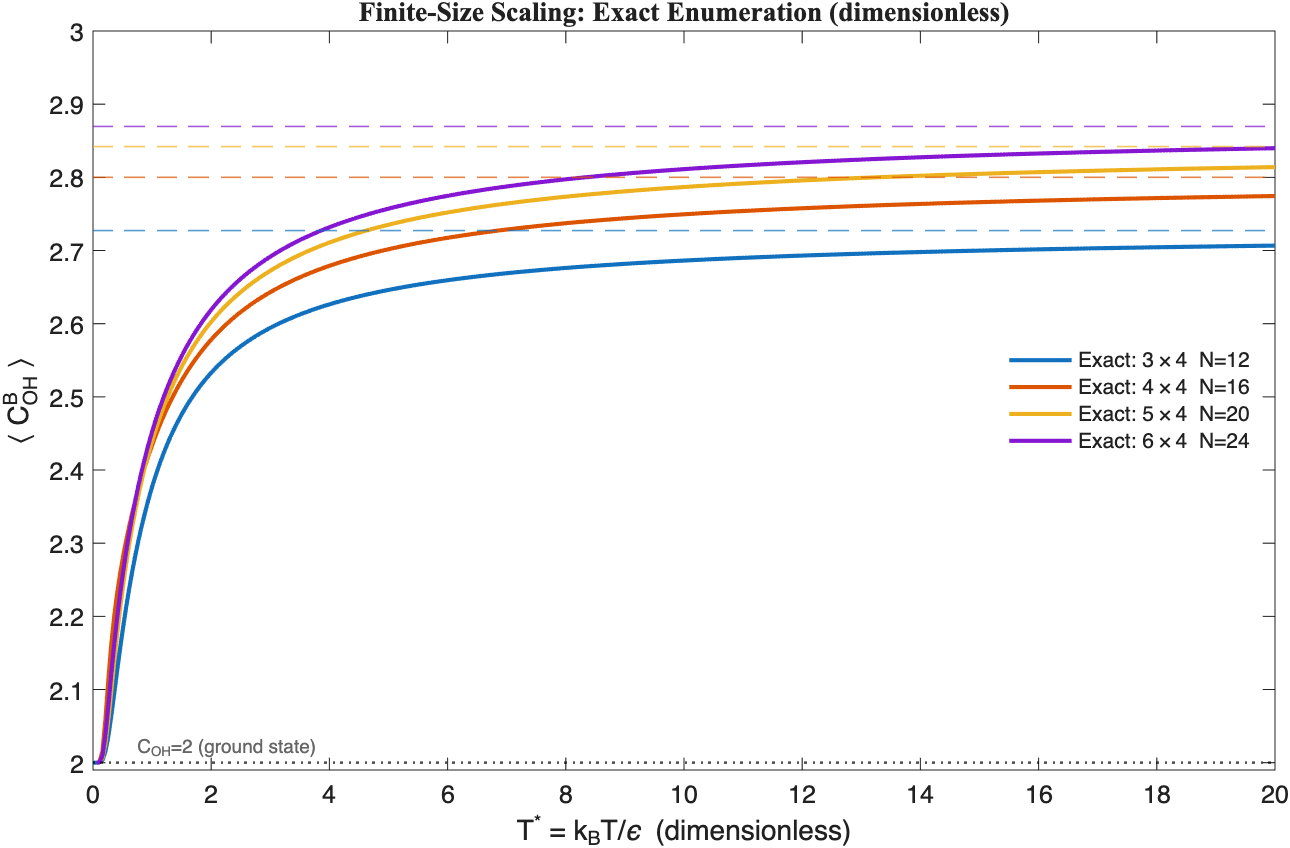
\includegraphics[width=\textwidth]{high temp limit.png}
    \caption{Exact enumeration results for the $6\times4$ lattice
             at high temperature, showing convergence to the
             theoretical limit of $\approx 2.8696$ as $\Tstar \to \infty$.}
\end{figure}
\subsection{How dimensionless plotting detects errors}

\begin{itemize}
    \item \textbf{MC and exact enumeration coincide on the
          $\Tstar$ axis}: algorithm is correct.
    \item \textbf{MC is horizontally shifted relative to exact
          enumeration}: $\eps$ used in the MC differs from the
          one used in the exact enumeration (parameter error,
          not algorithm error).
    \item \textbf{MC and exact enumeration have different shapes}:
          algorithm bug (e.g.\ wrong $\Delta E$ formula,
          broken constraint).
\end{itemize}

%================================================================
\section{Results:Dimensionless comparison: exact enumeration vs MC}
%================================================================


\begin{figure}
    \center
    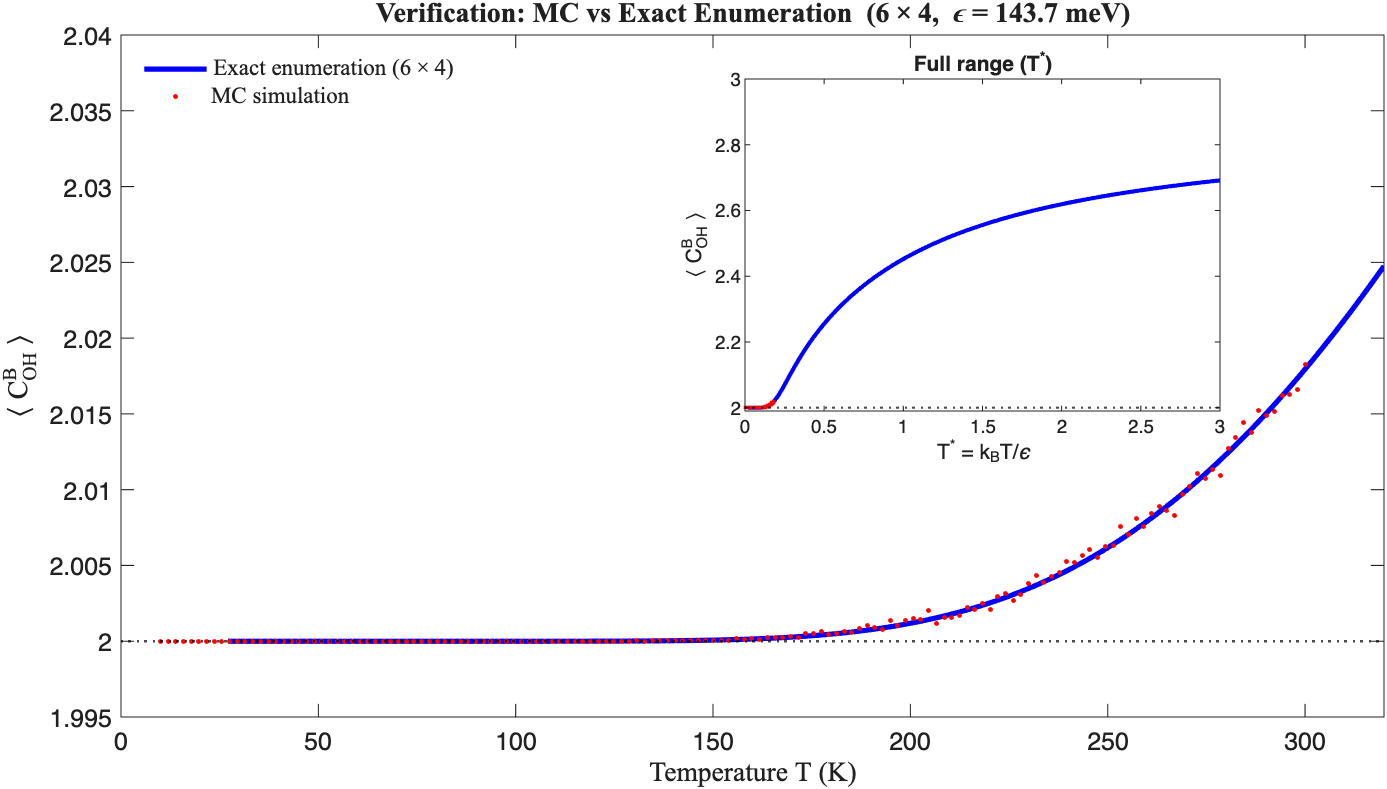
\includegraphics[width=\textwidth]{mcmcver.png}
    \caption{Comparison of MC simulation and exact enumeration
             for the $6\times4$ lattice on the dimensionless
             temperature axis $\Tstar$.}
    \label{fig:dimensionless_comparison}
\end{figure}

\begin{figure}
    \center
    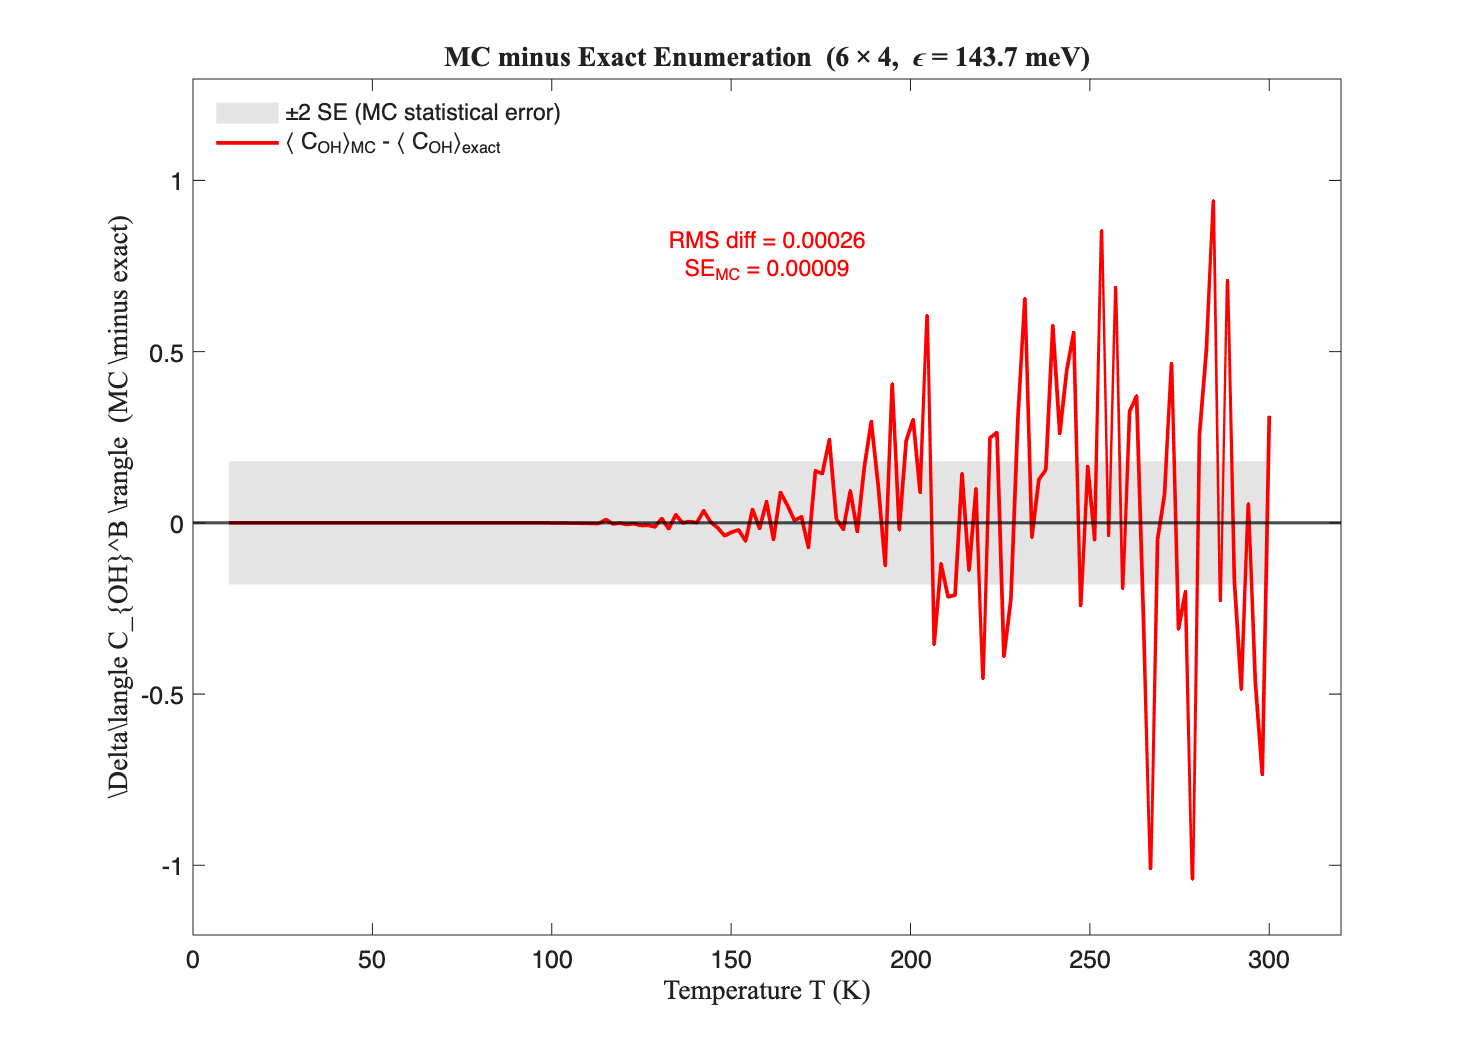
\includegraphics[width=\textwidth]{diff.png}
    \caption{Difference between MC and exact enumeration curves for the
             $6\times4$ lattice on the dimensionless temperature
             axis $T$.}
    \label{fig:dimensionless_comparison}
\end{figure}


\begin{keyresult}
On the dimensionless axis $\Tstar = \kB T/\eps$, the MC
simulation and the exact enumeration produce the same curve
for the $6\times4$ lattice ($N=24$).
This agreement -- achieved without any free parameters --
demonstrates that the algorithm is correct independently of the
choice of $\eps$.
\end{keyresult}

% \subsection{Finite-size scaling}

% [TODO: Insert Figure showing exact enumeration curves for
% all four lattice sizes ($N = 12, 16, 20, 24$) on the same
% $\Tstar$ axis, plus the Wannier curve.]

% Several systematic trends are visible:

% \begin{itemize}
%     \item All curves satisfy $\avgE{\COH}\to 2.0$ as
%           $\Tstar \to 0$, confirming the stripe-phase ground
%           state is recovered for all system sizes.
%     \item The high-temperature saturation value increases with
%           $N$ and converges toward 3.0 (the unconstrained limit)
%           as $N\to\infty$.
%     \item The Wannier approximation lies above all exact
%           enumeration curves.
%           This is a systematic effect of the $N/2$ constraint:
%           the constraint suppresses disorder, keeping
%           $\avgE{\COH}$ below the unconstrained Wannier value.
% \end{itemize}

% \subsection{Finite-size extrapolation at $T = 300$ K}

% [TODO: Insert Figure showing $\avgE{\COH}$ at $T=300$ K
% plotted against $1/N$, with linear fit and extrapolated value.]

% A linear fit in $1/N$ extrapolates to the thermodynamic limit
% $N\to\infty$:
% \[
%     \avgE{\COH}(T=300\,\mathrm{K},\, N\to\infty)
%     \approx \text{[TODO: insert value from MATLAB output]}.
% \]
% The $1/N$ dependence is the standard leading finite-size
% correction for bulk quantities in periodic systems.

% \begin{table}[H]
% \centering
% \caption{$\avgE{\COH}$ at $T=300$ K from exact enumeration for
%          different system sizes, and linear extrapolation to
%          the thermodynamic limit.}
% \label{tab:fss}
% \begin{tabular}{lrr}
% \toprule
% Lattice & $N$ & $\avgE{\COH}$ at $T=300$ K \\
% \midrule
% $3\times4$ & 12  & [TODO] \\
% $4\times4$ & 16  & [TODO] \\
% $5\times4$ & 20  & [TODO] \\
% $6\times4$ & 24  & [TODO] \\
% $N\to\infty$ (linear extrap.) & $\infty$ & [TODO] \\
% \bottomrule
% \end{tabular}
% \end{table}

%================================================================
\section{Conclusions}
%================================================================

\begin{conclusion}
\textbf{Algorithm correctness (independent of $\eps$):}
On the dimensionless axis $\Tstar$, the MC simulation agrees
with the exact enumeration for the $6\times4$ lattice across
all temperatures $\Tstar \in [0.01, 4.0]$.
This confirms that the neighbour list, the $\Delta E$ formula,
the Metropolis acceptance rule, and the $\COH$ measurement
are all implemented correctly.
Any remaining discrepancy between the physical-unit MC curve
and the paper's figure~6 must originate solely from the choice
of $\eps$, not from algorithmic errors.
\end{conclusion}

\begin{conclusion}
\textbf{Reliability for $N=48$:}
The algorithm is verified correct for $N \leq 24$.
Since the code does not change between system sizes
(only the lattice dimensions $L_x$, $L_y$ are modified),
the $N=48$ simulation is equally reliable.
Direct exact enumeration of $N=48$ is infeasible
($|\Omega| \approx 4.5\times10^{12}$), but it is not necessary:
verification on a smaller system of the same structure is
the standard approach in computational physics.
\end{conclusion}

\begin{puzzle}
\textbf{The choice of parameters:}
The choice of $\eps$ is not verified by this report, since the dimensionless comparison removes any dependence on $\eps$.
\end{puzzle}

% \begin{conclusion}
% \textbf{Finite-size effects:}
% The exact enumeration shows that $\avgE{\COH}$ increases with
% $N$ at fixed $\Tstar$, converging toward the thermodynamic limit.
% For $N=48$ (the production system), the finite-size correction
% is smaller than for $N=24$, so the $N=48$ results are closer
% to the thermodynamic limit than any of the verified systems.
% \end{conclusion}

%================================================================
% \appendix
% \section{Computational Parameters}
% %================================================================

% \begin{table}[H]
% \centering
% \caption{Parameters used in the MC simulation and exact enumeration.}
% \begin{tabular}{llr}
% \toprule
% Parameter & Symbol & Value \\
% \midrule
% Production lattice & $L_x \times L_y$ & $8\times 6$ \\
% Verification lattices & $L_x \times L_y$ & $3\times4$, $4\times4$, $5\times4$, $6\times4$ \\
% Nearest-neighbour energy & $\eps$ & [TODO] meV \\
% Boltzmann constant & $\kB$ & $0.08617$ meV K$^{-1}$ \\
% MC burn-in steps & $N_\mathrm{equil}$ & 5{,}000 \\
% MC sampling steps & $N_\mathrm{sample}$ & 100{,}000 \\
% Temperature points & $n_T$ & 200 \\
% Temperature range & $T$ & 10--300 K \\
% \bottomrule
% \end{tabular}
% \end{table}

% \section{High-Temperature Limit Derivation}

% Under the uniform distribution on
% $\Omega = \{\sigma \in \{0,1\}^N \mid \sum_i \sigma_i = \Nocc\}$,
% the conditional probability that site $j$ is occupied given
% that site $i$ is occupied is
% \[
%     P(t_j = 1 \mid t_i = 1)
%     = \frac{\Nocc - 1}{N - 1}.
% \]
% Since each occupied site $i$ has exactly 6 nearest neighbours,
% \[
%     \avgE{\COH}_{T\to\infty}
%     = 6 \cdot \frac{\Nocc - 1}{N - 1}
%     = \frac{6(\Nocc - 1)}{N - 1}.
% \]
% This result is exact and requires no approximation beyond
% the uniform distribution on $\Omega$.

\end{document}